\documentclass{article}
\usepackage[utf8]{inputenc}
\usepackage[english,serbian]{babel}
\usepackage{graphicx}
\usepackage{amsmath,amssymb}
\usepackage{siunitx}
\usepackage{float}
\usepackage[utf8]{inputenc}
\usepackage[unicode]{hyperref}
\usepackage[lofdepth,lotdepth]{subfig}

\title{Poređenje performansi i uspešnosti \textit{Structure from Motion} algoritama na hardveru drona}
\author{Luka Simić i Petar Marković}
\date{Mart 2019}


\begin{document}

\maketitle

\section{Uvod}
    \textit{Structure from Motion} (SfM) tehnika se koristi za procenjivanje trodimenzionalnog prostora na osnovu dvodimenzionalnih slika tog prostora. U poslednjih nekoliko godina je primenjivana na različite načine, između ostalog i u radu s bespilotnim letelicama, odnosno dronovima. Većina dronova u današnje vreme je opremljena kamerom, što ih čini jednom od najboljih tehnika pomoću kojih se, uz kombinaciju s \textit{Structure from Motion} tehnikom, može napraviti trodimenzionalni model nekog prostora.

    Dronovi mogu obavljati ovu operaciju na dva načina: ručno, pod kontrolom čoveka koji upravlja njihovim kretanjem i kamerom, ili automatski, korišćenjem izmerenih parametara za snalaženje drona u prostoru i određivanja mesta slikanja. Za drugi pristup mogu se koristiti različiti parametri, poput senzora razdaljine, stereo kamere, itd. ali dosta njih zahteva dodatnu nadogradnju (i nakon toga kalibraciju) drona. Cilj ovog projekta jeste da uporedi preciznost SfM varijacija koje performansama dovoljnim za korišćenje u realnom vremenu omogućavaju korišćenje samo kamere za snalaženje drona u prostoru uz pomoć SfM-a.

    \begin{figure}
        \centering
        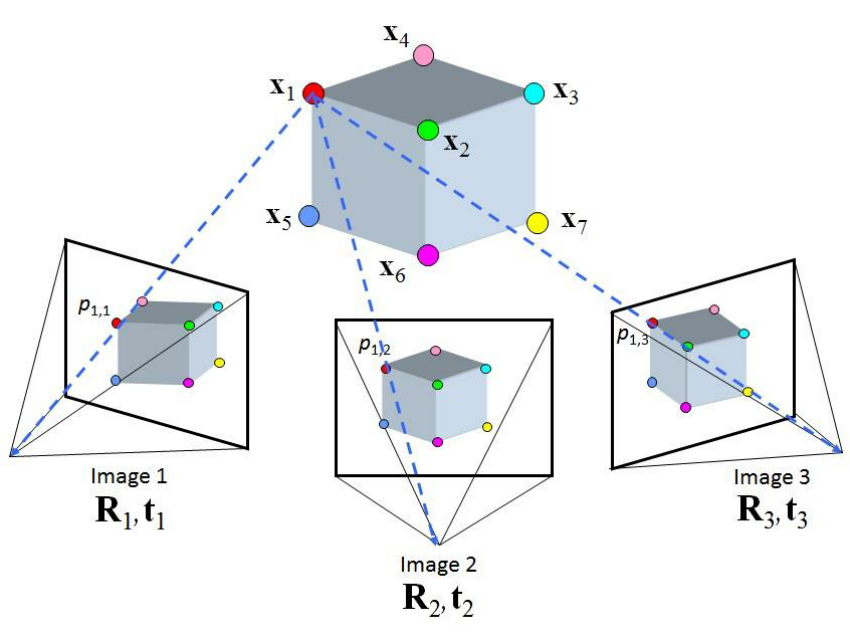
\includegraphics[scale=0.2]{SfM.png}
        \caption{Ilustracija rada \textit{Structure from Motion} tehnike. Dostupno na: \url{https://www.researchgate.net/figure/Structure-from-Motion-SfM-process-is-illustrated-The-structure-in-the_fig2_269327935} [Pristupano 2. marta 2019].}
        \label{SfM}
    \end{figure}

\section{Metod rada}
    % Treba nešto o načinu na koji će se hardver programirati.
    SfM se sastoji iz nekoliko etapa:
    \begin{itemize}
        \item Pronalaženje objekata za praćenje na slici (\textit{feature detection}),
        \item Povezivanje izabranih objekata između dve slike (\textit{feature tracking}),
        \item Rekonstrukcija modela prostora.
    \end{itemize}
    Za svaku od ovih etapa postoji više načina da se izvrše, i cilj ovog projekta jeste da uporedi performanse i uspešnosti njihovog izvršavanja u različitim uslovima. Upoređivanje performansi se može raditi prostim merenjem dužine izvršavanja etape, ali merenje uspešnosti metoda bi moralo ručno da se radi.

    % Slike za svaku od etapa.

    \subsection{Feature detection}
        Glavni cilj \textit{feature detection} algoritama jeste pronalaženja tački ili objekata (obično ivica ili ćoškova) od važnosti koje će kasnije biti od koristi \textit{feature tracking} algoritmima.

        Neki od poznatih \textit{feature detection} algoritama su:
        \begin{itemize}
            \item \textit{Harris Corner Detector} (prikazan na slici \ref{Harris})
            \item \textit{Features from Accelerated Segment Test} (FAST)
            \item \textit{Scale-Invariant Feature Transform} (SIFT)
            \item \textit{Speeded Up Robust Features} (SURF)
            \item \textit{Oriented FAST and Rotated BRIEF} (ORB)
        \end{itemize}
        \begin{figure}[H]
            \centering
            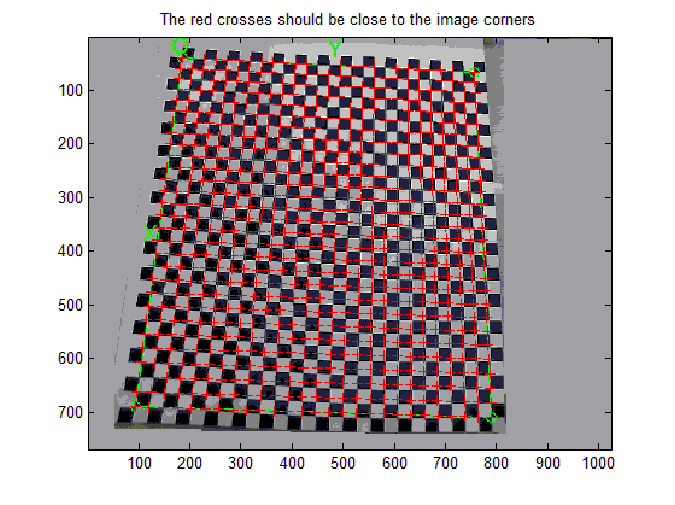
\includegraphics[width=0.8\textwidth]{Harris.png}
            \caption{Rad \textit{Harris Corner Detector}-a na šahovskoj tabli. Dostupno na: \url{https://www.researchgate.net/figure/Harris-corner-detection-for-the-checkerboard_fig4_308849698} [Pristupano 14. marta 2019].}
            \label{Harris}
        \end{figure}
    \subsubsection{SIFT}
    
    
    \subsection{Feature tracking}
        \textit{Feature tracking} algoritmi imaju za cilj praćenje objekata kroz različite slike. Mogu biti direktni i indirektni. Direktni \textit{feature tracking} algoritmi–poput \textit{Kanade–Lucas–Tomasi} (KLT, prikazan na slici \ref{KLT}) i raznih \textit{block-matching} algoritama–smenjuju \textit{feature detection} algoritme u potpunosti jer se njihove metode ne zasnivaju na prethodnoj detekciji objekata, dok indirektni koriste rezultate prethodne etape.

        \begin{figure}[H]
            \centering
            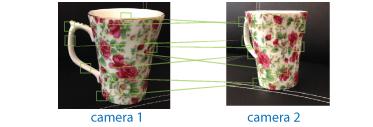
\includegraphics[scale=0.8]{KLT.png}
            \caption{KLT detektuje kako su se tačke jedne slike pomerile u drugoj. Dostupno na: \url{https://www.mathworks.com/help/vision/ug/structure-from-motion.html\#bu8chur-3} [Pristupano 14. marta 2019].}
            \label{KLT}
        \end{figure}

    \subsection{Rekonstrukcija}
        Kao poslednji korak SfM-a, povezane slike se moraju nekako rekonstruisati u 3D model prostora, i prilikom ove etape se najčešće koristi \textit{bundle adjustment}. \textit{Bundle adjustment} je metoda pomoću koje se popravljaju rezultati prethodnih etapa SfM-a. Generalno razlikujemo lokalan (između dve slike) i globalan (između svih slika) \textit{bundle adjustment}, ali postoje razni pristupi \textit{bundle adjustment}-u koji bi mogli da se porede međusobno.

    % \begin{figure}[H]
    %     \centering
    %     \subfloat[]{\includegraphics[width=0.5\textwidth]{SIFT.jpg}} \\

    %     \subfloat[]{\includegraphics[width=0.475\textwidth]{SIFT.jpg}}
    %     \subfloat[]{\includegraphics[width=0.475\textwidth]{SIFT.jpg}}
    %     \caption{Primeri rezultata etapa \textit{Structure from Motion}-a. Izvori: \url{http://aishack.in/tutorials/sift-scale-invariant-feature-transform-introduction/} [Pristupano 3. marta 2019], }
    % \end{figure}

\section{Istraživački rad}
    Glavni cilj istraživanja jeste da se uporede moguće kombinacije različitih algoritama u svakoj etapi, odredi najbolja od isprobanih kombinacija i, po mogućnosti, testira na realnom hardveru radi verifikacije.

    Upoređivanje će biti vršeno korišćenjem \textit{dataset}-ova iz \cite{dataset}. Performanse kombinacija algoritama će biti testirane merenjem dužine njihovog izvršavanja. Preciznost \textit{point cloud}-ova koje kombinacije algoritama generišu će biti merena uz pomoć \textit{Iterative closest point} (ICP) algoritma tako što\cite{stojke}:
    \begin{itemize}
        \item Uzmu se \textit{point cloud} generisan iz slika u \textit{dataset}-u ($G$) i referentni \textit{point cloud} iz \textit{dataset}-a ($R$).
        \item Pretpostavi se da je rotacija između $G$ i $R$ mala (jer su generisani iz istog seta slika).
        \item Odaberu se slučajne tačke za koje se onda izračuna najbolja transformacija (translacija ili rotacija) koja preslikava tačke iz $G$ u tačke iz $R$.
        \item Izračunata transformacija se obavi za sve tačke iz $G$.
        \item Od koraka 3 pa na dalje se ponavlja sve dok rastojanje između tačaka $G$ i $R$ ne bude dovoljno malo ili broj iteracija prevrši zadatu meru.
        \item Krajnja preciznost \textit{point cloud}-a (što predstavlja uspešnost algoritma) se računa kao zbir kvadrata rastojanja između tačaka iz $G$ i njima najbližih tačaka iz $R$.
    \end{itemize}
    Takođe bi kao istraživački rad bilo moguće dokazati ili opovrgnuti par hipoteza:
    \begin{itemize}
        \item Vreme izvršavanja će moći da se svede na ispod 100ms.
        \item Hardver neće moći da čuva ceo \textit{point cloud} dobijen SfM-om u svojoj memoriji.
    \end{itemize}

\begin{thebibliography}{2}
    \bibitem{featuredetection}
    Shimiao, L. (2017). \textit{A review of feature detection and match algorithms for localization and mapping}. [online] Dostupno na: \url{https://iopscience.iop.org/article/10.1088/1757-899X/231/1/012003} [Pristupano 2. marta 2019].
    \bibitem{featuretracking}
    Irani, M. \textit{et al.} (1999). \textit{All About Direct Methods}. [online] Dostupno na: \url{http://pages.cs.wisc.edu/~dyer/ai-qual/irani-visalg00.pdf} [Pristupano 3. marta 2019].
    \bibitem{bundleadjustment}
    Mouragnon, E. \textit{et al.} (2007). \textit{Generic and real-time structure from motion using local bundle adjustment}. [online] Dostupno na: \url{https://www.sciencedirect.com/science/article/pii/S0262885608002436} [Pristupano 2. marta 2019].
    \bibitem{dataset}
    Roberto, T. \textit{et al.} (2015). \textit{Hierarchical structure-and-motion recovery from uncalibrated images}. [online] Dostupno na: \url{https://arxiv.org/abs/1506.00395} [Pristupano 31. marta 2019].
    \bibitem{stojke}
    Stojanović, M. i Arbanas, M. (2012). \textit{Mapiranje prostora pomoću Turtlbota}. U: Petničke sveske 2012(1), str. 137–141.
\end{thebibliography}
\end{document}
